\subsection{Halved Model}


\begin{figure}
    \centering
    \subfloat[The full model]{
        \includegraphics[width=.4 \textwidth]{62_MinimalRepr_Adding/2D_Period_1_Zoomed/result.png}
    }
    \subfloat[The halved model]{
        \includegraphics[width=.4 \textwidth]{63_MinimalRepr_Adding_Halved/2D_Period_1_Zoomed/result.png}
    }
    \caption{
        2D period scans of a period adding regions of the same model in two different versions.
        On the left, is the full version of the model and on the right, is the halved version of the model.
        The red markers between the regions $P_{10}^4$ and $P_{10}^4 \oplus P_9^4$ in both pictures, is the parameter range used for the 1D scans in \Cref{fig:minrep.adding1.motivation.halved.1d.period}.
    }
    \label{fig:minrep.adding1.corner.period}
\end{figure}

\begin{figure}
    \centering
    \subfloat[The full model]{
        \includegraphics[width=.4 \textwidth]{62_MinimalRepr_Adding/1D_Period_1_add_hor_D1/result.png}
        \label{fig:minrep.adding1.motivation.halved.1d.period.full}
    }
    \subfloat[The halved model]{
        \includegraphics[width=.4 \textwidth]{63_MinimalRepr_Adding_Halved/1D_Period_1_add_hor_D1/result.png}
    }
    \caption{
        1D period scans of a period-adding cascade of the same model in two different versions.
        On the left, is the full version of the model and on the right, is the halved version of the model.
        The parameter range is the same in both models and is marked red in \Cref{fig:minrep.adding1.corner.period}.
    }
    \label{fig:minrep.adding1.motivation.halved.1d.period}
\end{figure}

Problems with \Cref{fig:minrep.adding1.motivation.halved.1d.period.full}:
\begin{itemize}
    \item The period of $\sigma\rho$ is more than the periods of $\sigma$ and $\rho$ combined
    \item The period of $\sigma^2\rho$ is smaller than the period of $\sigma\rho$
\end{itemize}

In the full model: $\sigma = \A^6\B^4\C^6\D^4$ (Period 20) and $\rho = \{\A^6\B^4\C^5\D^4, \A^5\B^4\C^6\D^4\}$ (Period 19).
If we glue the cycles together, we would expect $\sigma\rho = \{\A^6\B^4\C^6\D^4\A^6\B^4\C^5\D^4, \A^6\B^4\C^6\D^4A^5\B^4\C^6\D^4\}$ (Period 39).
But when we simulate the full model at this point, we get only one cycle $\sigma\rho = \A^5\B^4\C^6\D^4\A^6\B^4\C^5\D^4\A^6\B^4\C^6\D^4$ with period 58.

Explanation: What is actually happening is that the cycles $\sigma = \L^6\R^4$ (Period 10) and $\rho = \L^6\R^4\L^5\R^4$ (Period 19) of the halved model get glued together.
In the full model, they manifest as the cycles $\sigma$ and $\rho$ described in the last section.
The resulting cycle is $(\L^6\R^4)^2\L^5\R^4 \equiv \L^6\R^4\L^6\R^4\L^5\R^4$
This cycle manifests as $\sigma\rho = \A^5\B^4\C^6\D^4\A^6\B^4\C^5\D^4\A^6\B^4\C^6\D^4$ in the full model.

Therefore, the cycle $\rho \equiv \L^6R^4\L^5\R^4$ itself is the two cycles $\sigma \equiv \L^6\R^4$ and $\rho' \equiv \L^5\R^4$ glued together.
\Cref{fig:tree.adding1.hor.halved} shows the farey tree of this adding cascade of $\sigma$ and $\rho'$ in the halved model up to level 4.
\Cref{fig:tree.adding1.hor.full} shows the farey tree of the same adding cascade, but this time the symbolic sequences are in the full model.
The adding is not apparent at all, since the cycles do not get glued together in the full model.
How to translate cycles between the different model flavors is discussed in the following.

\subsubsection{Translating Cycles}

We can get the manifestation of a cycle from the halved system in the full system by ``unrolling'' the cycle.
For this, we write down the cycle of the halved model three times in a row.
For our cycle $\sigma\rho$ this would be $\L^6\R^4\L^6\R^4\L^5\R^4|\L^6\R^4\L^6\R^4\L^5\R^4|\L^6\R^4\L^6\R^4\L^5\R^4$.
Then we make pairs on rotations until the next pair would start at the same point, the first pair started in the original cycle.
This step has to be repeated with every rotation of the original cycle as the starting position once.
For the first iteration, we start with the first rotation.
In our example, we would get the pairs $\L^6\R^4\L^6\R^4$, $\L^5\R^4\L^6\R^5$, and $\L^6\R^4\L^5\R^4$.
Here we stop, because the next pair would start at the beginning of the original cycle in the halved model.
For each pair, we replace the first $\L$ by $\A$, the first $\R$ by $\B$, the second $\L$ by $\C$, and the second $\R$ by $\D$ and put them toghether again.
In our example, we get $\A^6\B^4\C^6\D^4\A^5\B^4\C^6\D^4\A^6\B^4\C^5\D^4$, which is exactly what we got in the simulation.

For the second iteration, we would get the pairs $\L^6\R^4\L^5\R^4$, $\L^6\R^4\L^6\R^4$, and $\L^5\R^4\L^6\R^4$.
This results in $\A^6\B^4\C^5\D^4\A^6\B^4\C^6\D^4\A^5\B^4\C^6\D^4$, which is equivalent to the result of the last paragraph by rotating it one complete rotation in the full model.
The third iteration also produces the same cycle rotated one time and is omitted here.

The inverse, ``rolling'' is easier.
We just write down the cycle in the full model, for example, $\A^6\B^4\C^6\D^4$.
Then we replace $\A$ and $\C$ by $\L$, and $\B$ and $\D$ by $\R$.
In our example, we get $\L^6\R^4\L^6\R^4$.
Last, we need to remove redundancy.
In our example, the cycle repeats itself twice, so we remove one half and get the result $\L^6\R^4$.

\subsubsection{$\sigma^2\rho$}

Now equipped with this tool, we can try to explain the cycle at $\sigma^2\rho$.
In both trees, \Cref{fig:tree.adding1.hor.halved,fig:tree.adding1.hor.full}, the node for this cycle is the lowest node on level 3.
The cycle in the halved model is $(\L^6\R^4)^3\L^5\R^4$ as expected of period adding.
In the full model, this cycle manifests as two coexisting cycles, $\A^6\B^4\C^6\D^4\A^6\B^4\C^5\D^4$ and $\A^6\B^4\C^6\D^4\A^6\B^4\C^5\D^4$.
These are exactly the cycles we get when simulating the full model at this point.

\begin{figure}
    \centering
    \includegraphics[width=\textwidth]{FareyTrees/Minrep_Adding1_Halved/adding.png}
    \caption{t}
    \label{fig:tree.adding1.hor.halved}
\end{figure}

\begin{figure}
    \centering
    \includegraphics[width=\textwidth]{FareyTrees/Minrep_Adding1_Full/adding.png}
    \caption{t}
    \label{fig:tree.adding1.hor.full}
\end{figure}